% =====================================================================
% Reponses aux questions .bis du mail de l'encadrant du 15 septembre 2026.
%
% Document NEUF et SEPARE : il ne modifie aucun livrable existant. Le rapport
% final et les redactions redaction_Q*.tex restent en l'etat.
%
% Langue : francais. Le mail de l'encadrant est en francais et ce document doit
% d'abord se comprendre ; la mise a l'anglais suivra s'il rejoint le rapport.
%
% Tout est recalcule HORS LIGNE par resultats_R2/scripts/analyse_bis.py depuis
% les Parquet de la campagne. Une seule exception, declaree en section 5 : le
% pilote instrumente par arbre (exp_bis_pilote_arbres.py), qui est une campagne
% et non une verification.
%
% Compiler depuis 04_experimentations/ :  latexmk -pdf reponses_questions_bis.tex
% Controle des chiffres :
%   python resultats_R2/scripts/verif_chiffres_tex.py reponses_questions_bis.tex
% =====================================================================

\documentclass[11pt,a4paper]{article}

\usepackage[utf8]{inputenc}
\usepackage[T1]{fontenc}
\usepackage[french]{babel}
\usepackage{amsmath,amssymb}
\usepackage[top=1.5cm,bottom=1.8cm,left=2cm,right=2cm]{geometry}
\usepackage{graphicx}
\usepackage{booktabs}
\usepackage{hyperref}
\hypersetup{colorlinks=true,linkcolor=black,citecolor=blue,urlcolor=blue}

\title{Questions complémentaires du 15 septembre :\\
profil d'erreur, fenêtre d'accumulation, matrice de corrélation}
\author{}
\date{}

\begin{document}
\maketitle

\section*{Cadre}

Ce document répond au mail du 15 septembre 2026, reproduit dans
\texttt{01\_consignes/Questions\_bis\_15sept.md}. Il ne modifie rien du rapport ni des
rédactions déjà rendues : il s'ajoute à elles.

Les énoncés complets des cinq questions n'ont pas été lus. Le fichier reçu est le corps du
mail rendu en HTML, et c'est la seule pièce jointe parvenue au groupe. Les réponses suivent
donc le texte du mail, question par question, dans l'ordre de priorité qu'il donne :
C.3.bis, C.2.bis, D.3.bis, D.1.bis, C.1.bis.

Tout est recalculé hors ligne par \texttt{resultats\_R2/scripts/analyse\_bis.py} depuis les
Parquet de la campagne de $2\,000$ exécutions (20 amplitudes $\times$ 100 graines,
horizon $H = 2\,000$ pas, forêt de $M = 10$ arbres, $\delta_P = 0.01$). Aucune
simulation n'a été relancée, à une exception près, annoncée en section~\ref{sec:d1bis} :
la variance entre arbres n'était calculable depuis aucune table, et un pilote instrumenté
a été lancé pour elle. Chaque chiffre cité se lit dans une table
\texttt{QCD\_bis\_*.parquet} nommée en note à sa première occurrence.

\paragraph{Notation.} Les nombres suivent la notation décimale du reste du dépôt, point
décimal, pour que le contrôle de traçabilité \texttt{verif\_chiffres\_tex.py} s'applique à ce
document sans être modifié. Le reste de la notation est celle du rapport, sans changement : $\tau_{\mathrm{ARF}}$ date du
premier remplacement d'arbre, $\tau_{\mathrm{swap}}(q)$ date du renouvellement d'une
fraction $q$ de la forêt, $\tau_{\mathrm{det}}$ date de l'alarme du détecteur,
$A(H)$ aire d'erreur excédentaire sur l'horizon complet, $A(0,w)$ la même sur la fenêtre
courte, $S_{\max}(H)$ statistique du détecteur, $\hat{p}_0$ socle d'erreur pré-rupture
estimé sur $3\,000$ pas, $\Delta e$ amplitude du changement.

\paragraph{Ce que le mail change au cadre.} L'encadrant tranche que $A$ est la métrique de
référence de l'adaptation du classifieur, $S_{\max}$ restant celle du détecteur. Les
questions ci-dessous adoptent cette lecture. Elle est compatible avec la réponse de la
question~D du rapport, qui sépare déjà les deux : $\tau_{\mathrm{ARF}}$ ne dit rien de
$A(H)$ et porte une association faible avec $S_{\max}(H)$.

\section{C.3.bis : le profil d'erreur après la rupture}

\paragraph{Réponse.} L'erreur décroît d'un niveau de départ mesuré vers un palier $e_\infty$
qui n'est pas $\hat{p}_0$ : il passe en dessous aux vingt amplitudes, et l'écart dépasse deux
erreurs types aux trois plus fortes. Le temps caractéristique de cette décroissance ne suit
ni $\tau_{\mathrm{ARF}}$ ni la loi $18.5\,\Delta e^{-0.98}$ de l'article. Il dépasse
$\tau_{\mathrm{ARF}}$ médian sur $17$ des $18$ amplitudes lisibles, d'un facteur $0.8745$ à
$1.5625$, mais l'intervalle de confiance de $t_{1/2}$ ne l'en sépare que sur $8$ d'entre
elles : l'énoncé prudent est que les deux horloges sont du même ordre, avec un avantage à
$t_{1/2}$. Contre la loi de l'article, le rapport passe de $1.822$ à $\Delta e = 0.141$ à
$0.818$ à $\Delta e = 0.498$ : elle est trop courte en bas de grille et trop longue en haut.
Enfin le profil n'est pas exponentiel là où sa forme est mesurable : le rapport
$t_{90}/t_{1/2}$ y vaut $1.4839$ à $1.8286$, contre $\ln 10 / \ln 2 = 3.3219$.

\subsection{Définitions, posées avant les mesures}

Le profil moyen $\bar{e}_t$ est la moyenne sur les 100 graines de l'amplitude, sans aucun
lissage temporel : un filtre de longueur $L$ décale tout marqueur de $L/2$, et la table ne
porte donc que la moyenne inter-graines.

Le palier $e_\infty$ est la moyenne de $\bar{e}_t$ sur la fenêtre $[1500 ; 2000)$,
\emph{déclarée avant mesure} et disjointe du transitoire. Elle reproduit exactement, à
$3.5 \cdot 10^{-18}$ près, la colonne \texttt{erreur\_fin\_horizon} de
\texttt{QCD\_fin\_horizon\_full} à la fenêtre 500, ce qui sert de contrôle de
non-régression.\footnote{\texttt{QCD\_bis\_profil\_erreur.parquet},
\texttt{QCD\_bis\_demi\_vie.parquet}.} Sa fiabilité est testée par amplitude : l'écart entre
les moyennes sur $[1500 ; 1750)$ et $[1750 ; 2000)$ est comparé à deux fois son erreur type
inter-graines. Deux amplitudes sur vingt échouent ce test, $\Delta e = 0.390998$ et
$\Delta e = 0.465040$ ; leurs lignes restent dans la table, marquées, et la
section~\ref{sec:nonfait} dit ce que cela coûte.

Le niveau de départ $e_{\mathrm{start}}$ est \emph{mesuré}, moyenne de $\bar{e}_t$ sur
$[0 ; 5)$, soit 500 observations. La valeur théorique $\hat{p}_0 + \Delta e$ ne sert que de
colonne de contrôle : le rapport a déjà établi qu'elle est réfutée sur les vingt amplitudes,
et l'employer au dénominateur fabriquerait un temps de demi-vie là où il n'y en a pas.

Le temps de fraction $t_q$ est le premier instant où la moyenne de $\bar{e}$ sur une fenêtre
de 20 pas passe sous $e_\infty + (1-q)\,(e_{\mathrm{start}} - e_\infty)$. Il porte un
indicateur de lisibilité par fraction : $t_q$ ne se cite que si la marge
$(1-q)(e_{\mathrm{start}} - e_\infty)$ dépasse deux erreurs types au niveau franchi. Pour
$q = 0.50$, deux amplitudes échouent, $\Delta e = 0.028$ et $\Delta e = 0.085$ ; pour
$q = 0.90$, douze.

\subsection{Pourquoi la règle de persistance a dû changer}
\label{sec:persistance}

La règle appliquée dans le projet jusqu'au 15 septembre exige qu'un seuil soit franchi et
\emph{tenu 20 pas consécutifs}. Sur le cas synthétique où la réponse est connue, un
transitoire exponentiel de constante $\theta = 100$ dont la demi-vie vaut
$\theta \ln 2 = 69.3147$, elle donne $t_{1/2} = 112$, soit $62\%$ de trop. La cause est que
le bruit binomial à 100 graines vaut environ $\pm 0.038$ au niveau franchi : un seul pas
au-dessus du seuil casse la fenêtre, et l'instant retenu attend que la courbe soit descendue
bien plus bas.

La règle appliquée ici est le franchissement \emph{en moyenne} sur la même fenêtre de 20 pas.
C'est toujours une persistance, un pas isolé ne déclenche rien, mais le bruit y est divisé
par $\sqrt{20}$. Sur le même tirage, elle donne $t_{1/2} = 62$ pour la même vérité de
$69.3147$.\footnote{\texttt{QCD\_bis\_self\_check.parquet}, contrôle
\texttt{C2bis\_a2\_bernoulli}, lignes \texttt{t\_half\_regle\_pas\_a\_pas} et
\texttt{t\_half}.} Les deux valeurs sont dans la table, l'ancienne règle comme la nouvelle :
c'est ce contrôle qui a fait changer d'estimateur, et le biais résiduel, de l'ordre de la
moitié de la fenêtre de persistance, vaut pour toutes les valeurs de $t_q$ publiées ici.

\subsection{Ce que donne la mesure}

\begin{table}[htbp]
  \centering
  \begin{tabular}{lrrrrrr}
    \toprule
    $\Delta e$ & $e_{\mathrm{start}}$ & $e_\infty$ & $t_{25}$ & $t_{1/2}$ & $t_{90}$
    & $\tau_{\mathrm{ARF}}$ médian \\
    \midrule
    $0.028$ & $0.0240$ & $0.022040$ & $99$  & $296$ & $303$ & $118$ \\
    $0.141$ & $0.1260$ & $0.021420$ & $110$ & $230$ & $608$ & $263$ \\
    $0.287$ & $0.2940$ & $0.019080$ & $51$  & $100$ & $222$ & $64$  \\
    $0.498$ & $0.5060$ & $0.002440$ & $23$  & $30$  & $45$  & $28$  \\
    \bottomrule
  \end{tabular}
  \caption{Quatre amplitudes représentatives. La ligne $\Delta e = 0.028$ est donnée pour
  mémoire : ses trois temps de fraction échouent au test de lisibilité. La table complète, à
  vingt amplitudes, avec les intervalles de confiance bootstrap et les indicateurs, est dans
  \texttt{QCD\_bis\_demi\_vie.parquet}.}
\end{table}

À $\Delta e = 0.498$, $t_{1/2} = 30$ pas, intervalle $[28 ; 32]$, contre un
$\tau_{\mathrm{ARF}}$ médian de $28$ pas et une prédiction de l'article de $36.659$. À
$\Delta e = 0.141$, $t_{1/2} = 230$ pas, intervalle $[166 ; 304]$, contre un
$\tau_{\mathrm{ARF}}$ médian de $263$ et une prédiction de $126.209$. C'est la seule
amplitude lisible où $t_{1/2}$ passe \emph{sous} $\tau_{\mathrm{ARF}}$, et elle suffit à
interdire la formule « le profil est partout plus lent que le premier remplacement ».

Un intervalle bootstrap sur un instant de franchissement n'a de sens que si l'instant est
défini dans la plupart des rééchantillons. Le taux de rééchantillons sans franchissement est
publié avec chaque intervalle : il vaut $0.0000$ aux dix-neuf amplitudes à partir de
$\Delta e = 0.085$, pour les trois fractions, et $0.3980$ à $\Delta e = 0.028$.

Le palier mérite d'être lu pour lui-même. $e_\infty$ est inférieur à $\hat{p}_0$ aux vingt
amplitudes, mais l'écart n'excède deux erreurs types qu'aux trois plus fortes ; il y culmine
à $z = 4.1896$ pour $\Delta e = 0.498$, où $e_\infty = 0.002440$ contre un socle
$\hat{p}_0 = 0.023110$. L'erreur finit alors à un dixième de son niveau d'avant la rupture.
C'est l'acquis déjà consigné selon lequel la tâche devient plus facile après le changement,
et il interdit de lire $A(H)$ comme une quantité d'erreur subie.

\subsection{La forme du profil}

Le test de forme n'est pas le recalage des courbes en $t/t_{1/2}$ : toute courbe y passe par
$0.5$ en $x = 1$ par construction, et valider une métrique par une autre qui lui est liée est
le piège recensé au journal. La figure du recalage est donnée pour l'illustration, et
légendée comme telle.

Le test est le rapport $t_{90}/t_{1/2}$. Pour une exponentielle pure il vaut exactement
$\ln 10 / \ln 2 = 3.3219$. Sur les huit amplitudes où $t_{90}$ est lisible, il vaut de
$1.4839$ à $1.8286$, et la borne haute la plus élevée des huit intervalles de confiance est
$1.9714$. La valeur $3.3219$ est donc exclue partout où la forme est mesurable : le profil
décroît plus vite qu'une exponentielle en fin de transitoire.

Ce verdict porte une faiblesse qu'il faut écrire avec lui. Le rapport $t_{90}/t_{1/2}$
\emph{décroît} avec l'amplitude, corrélation de Spearman $-0.5107$ pour $p = 0.0214$, et le
critère de lisibilité ne se lève lui aussi qu'en haut de grille, parce que la marge
$0.1\,(e_{\mathrm{start}} - e_\infty)$ y croît tandis que $2\,se$ reste plat. Le tri et
l'effet vont donc dans le même sens, et les huit amplitudes retenues sont précisément celles
où le rapport est le plus bas : sa moyenne y vaut $1.6066$ contre $2.3385$ aux douze autres.
Aux deux amplitudes immédiatement inférieures au seuil, $\Delta e = 0.326793$ et
$\Delta e = 0.361418$, l'intervalle de confiance du rapport \emph{contient} $3.3219$. Le
compte de huit est lui-même fragile : le rapport de la marge à $2\,se$ vaut $1.0056$ à
$\Delta e = 0.465040$ et $0.9774$ à $\Delta e = 0.452271$, de sorte que deux décimales de
bruit le feraient basculer entre sept et neuf.

Ce qui est établi est donc étroit : \emph{aux amplitudes les plus fortes}, le profil n'est
pas exponentiel. Aux douze autres, la forme n'est pas distinguable d'une exponentielle sous
ce protocole, et rien ne permet d'étendre le verdict.

\subsection{Le témoin sans drift}

Sur les $2\,000$ exécutions sans rupture, $e_{\mathrm{start}} = 0.020700$ et
$e_\infty = 0.022843$ : la baisse mesurée est \emph{négative}, $-0.002143$. Aucun $t_q$ n'est
défini et aucun indicateur de lisibilité ne se lève. L'estimateur ne fabrique pas de
dynamique là où il n'y en a pas. Ce témoin tourne sur $2\,000$ graines quand la mesure en
utilise 100 par strate : son bruit est $\sqrt{20}$ fois plus faible, et il ne teste donc pas
le régime exact dans lequel $t_q$ est calculé.

\begin{figure}[htbp]
  \centering
  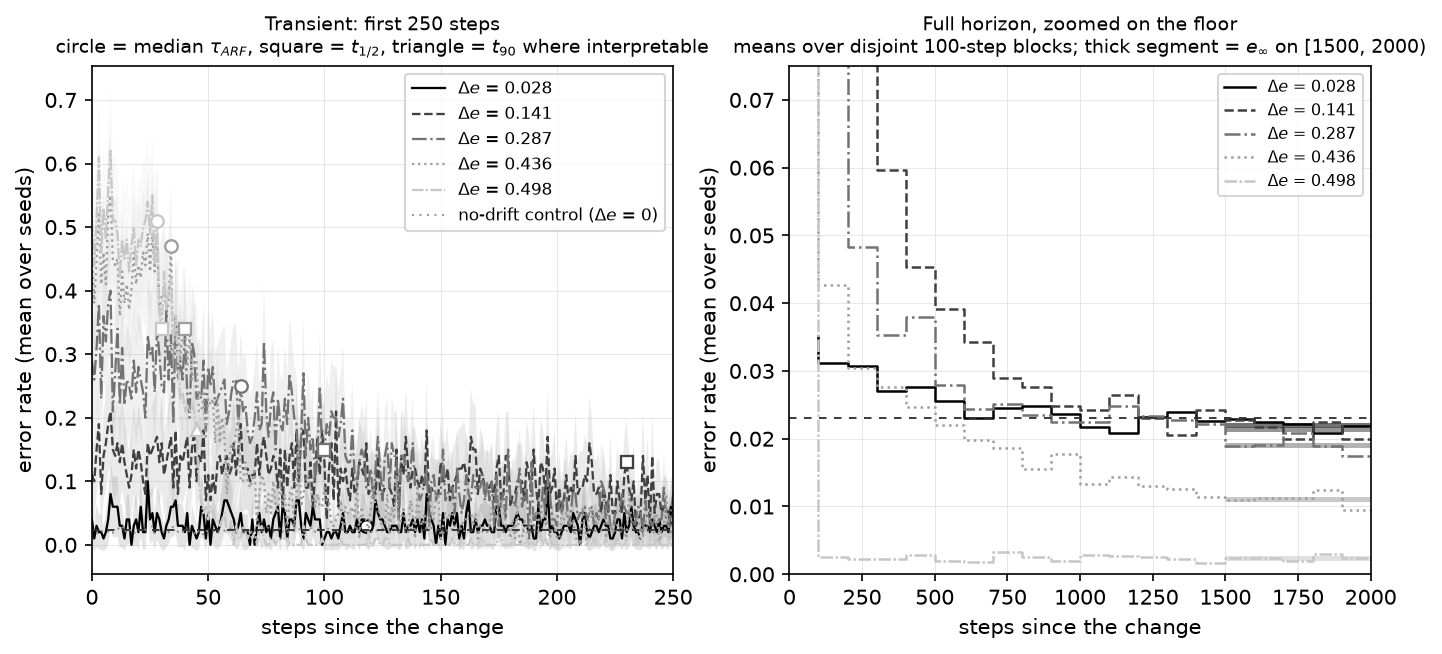
\includegraphics[width=\textwidth]{resultats_R2/resultats/figures/Fig_bis_profil_erreur.png}
  \caption{Profil d'erreur post-rupture. À gauche le transitoire, avec les marqueurs
  $\tau_{\mathrm{ARF}}$ médian, $t_{1/2}$ et $t_{90}$. À droite l'horizon complet en
  moyennes par blocs disjoints de 100 pas, qui montre le palier passant sous $\hat{p}_0$
  aux fortes amplitudes.}
\end{figure}

\begin{figure}[htbp]
  \centering
  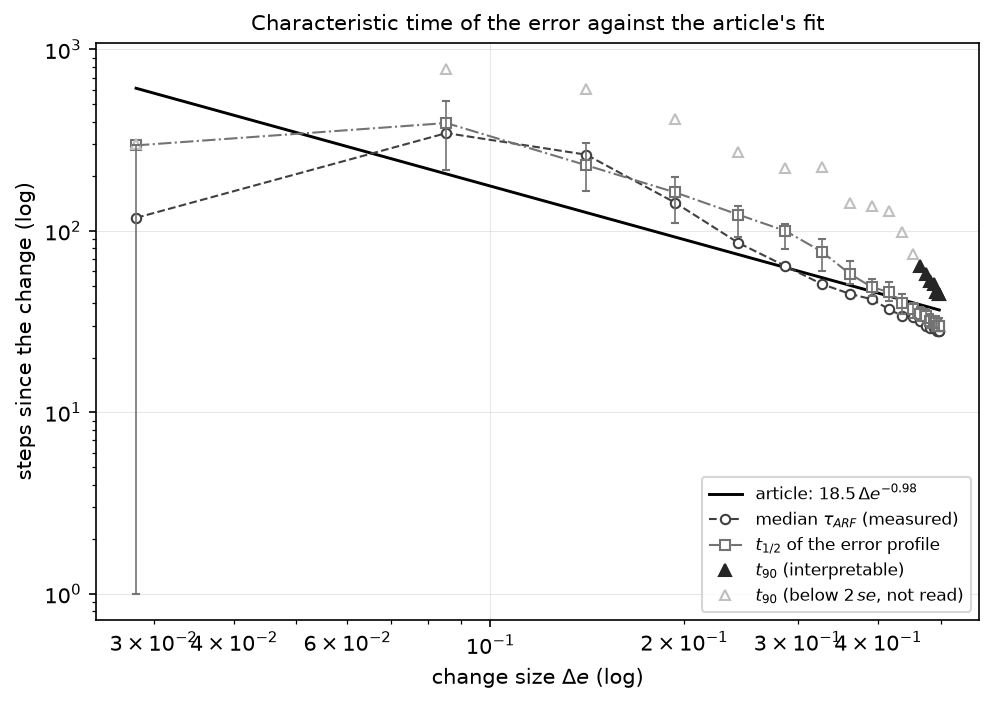
\includegraphics[width=0.78\textwidth]{resultats_R2/resultats/figures/Fig_bis_demi_vie_vs_article.png}
  \caption{Le pont avec l'article. $t_{1/2}$ dépasse $\tau_{\mathrm{ARF}}$ médian sur $17$
  des $18$ amplitudes lisibles ; l'exception, $\Delta e = 0.141$, est visible sur la figure,
  où la courbe de $\tau_{\mathrm{ARF}}$ passe au-dessus de celle de $t_{1/2}$. La loi
  $18.5\,\Delta e^{-0.98}$ coupe les deux.}
\end{figure}

\begin{figure}[htbp]
  \centering
  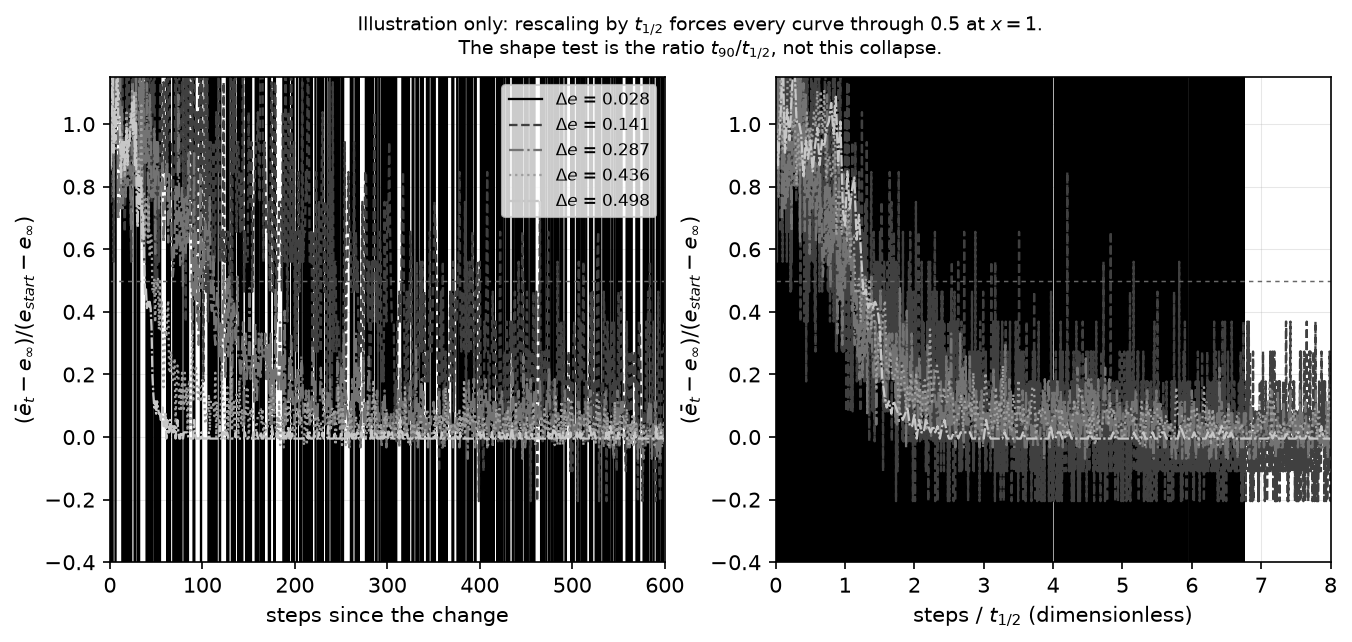
\includegraphics[width=\textwidth]{resultats_R2/resultats/figures/Fig_bis_profil_collapse.png}
  \caption{Illustration seulement. Le recalage par $t_{1/2}$ force toutes les courbes à
  passer par $0.5$ en $x = 1$ ; il ne teste pas la forme.}
\end{figure}

\clearpage

\section{C.2.bis : quelle fenêtre $w$ pour $A(0,w)$}
\label{sec:c2bis}

\paragraph{Réponse.} Le rapport signal sur bruit de $A(0,w)$ a bien un maximum intérieur, et
l'intuition du mail est confirmée : prolonger l'accumulation noie l'adaptation. Mais la
réponse n'est pas une fenêtre, c'est un intervalle. La fenêtre de certificat imposée par
l'énoncé, $w = 3 \cdot 18.5 / \Delta e$, est trop longue sur dix-neuf amplitudes sur vingt :
elle vaut $1.77$ à $2.49$ fois $w_{\mathrm{opt}}$ sur le haut de la grille,
$\Delta e \geq 0.4$, et $3.978$ fois à $\Delta e = 0.028$. Elle est en revanche plus
\emph{courte} que $w_{\mathrm{opt}}$ à $\Delta e = 0.141$, où le rapport vaut $0.885$, et ce
contre-exemple interdit d'en faire une règle. Au-delà d'un certain $w$, en haut de grille,
$\mu(w)$ change de signe et le rapport devient négatif : accumuler plus longtemps ne dégrade
pas seulement la mesure, elle en inverse le sens.

\subsection{Le cadre}

Avec $A(0,w) = \sum_{t=0}^{w-1} (e_t - \hat{p}_0)$, l'espérance
$\mu(w) = \sum_{t<w} (\bar{e}_t - \hat{p}_0)$ croît pendant le transitoire puis plafonne au
milieu de la grille, où $e_\infty \approx \hat{p}_0$, et \emph{décroît} en haut de grille, où
$e_\infty < \hat{p}_0$. Le contrôle de non-régression est immédiat : $A(0,2000)$ reproduit la
colonne \texttt{A\_H} de \texttt{QCD\_indicateurs\_full} à $6.0 \cdot 10^{-12}$
près.\footnote{\texttt{QCD\_bis\_snr\_fenetre.parquet}, \texttt{QCD\_bis\_w\_opt.parquet},
\texttt{QCD\_bis\_A0w\_par\_run.parquet}.}

La variance est mesurée sur les graines, et rien d'autre. La formule binomiale
$\sum_t \bar{e}_t(1-\bar{e}_t)$ est fausse sur ces données : le rapport de l'écart-type
empirique à cet écart-type théorique vaut $0.6001$ à $w = 50$ et $1.5866$ à $w = 2000$ pour
$\Delta e = 0.498$. Une forêt qui apprend produit une erreur autocorrélée et un effet de
graine que la formule ignore dans les deux sens. Elle ne sert ici qu'à l'illustration.

Le rapport $\mathrm{SNR}(w) = \mu(w)/\sigma(w)$ a un maximum intérieur. C'est la
formalisation de l'accumulation prolongée qui noie le transitoire. Dans le cas fermé d'un
transitoire exponentiel $\bar{e}_t - \hat{p}_0 = \Delta e\, e^{-t/\theta}$ avec un bruit
d'écart-type \emph{constant}, on a $\mathrm{SNR}(w) \propto (1 - e^{-w/\theta})/\sqrt{w}$,
maximal en $w_{\mathrm{opt}} = 1.2564\,\theta$, racine de $2x e^{-x} = 1 - e^{-x}$.

\subsection{Pourquoi ce cas fermé ne suffit pas}

Le contrôle sur cas connu sépare deux situations que le cadre confondait. Avec un bruit
additif d'écart-type constant, la formule s'applique et l'intervalle $W_{95}$ estimé sur 100
graines, $[110 ; 230]$, contient bien la vérité $125.64$. Avec des tirages de Bernoulli, dont
la variance $p_t(1-p_t)$ décroît avec le transitoire, la vérité calculée sur $20000$ graines
vaut $285$, soit $2.85\,\theta$ et non
$1.2564\,\theta$.\footnote{\texttt{QCD\_bis\_self\_check.parquet}.} La formule fermée ne
transporte donc pas sur des données binaires, et la fenêtre qu'elle suggère est \emph{plus
courte} que l'optimum, d'un facteur voisin de deux sur ce cas.

À 100 graines, l'argmax seul n'a de toute façon pas de contenu : sur le témoin à bruit
corrélé, la largeur de $W_{95}$ vaut $0.8462$ fois $w_{\mathrm{opt}}$. La lecture porte donc
sur $W_{95} = \{w : \mathrm{SNR}(w) \geq 0.95 \max\}$, dont la couverture est validée sur
100 réplications de 100 graines : l'intervalle bootstrap contient la vérité dans $0.9700$ des
cas et intersecte le $W_{95}$ vrai dans $1.0000$ des cas.

Ce témoin à bruit corrélé ne reproduit qu'en partie le régime des données. Son rapport
d'écart-type empirique à écart-type binomial vaut $0.9665$ à $w = 50$ et $2.0582$ à
$w = 2000$, quand les données donnent $0.6001$ et $1.5866$. Le sens est le bon, sous $1$ en
fenêtre courte et au-dessus en fenêtre longue, mais l'amplitude ne l'est pas : la couverture
validée sur ce témoin ne transporte donc pas telle quelle.

Le témoin sans signal lève bien son drapeau, mais pas par le critère prévu. Les deux critères
du plan, $w_{\mathrm{opt}}$ sur une borne de la grille et $W_{95}$ couvrant la moitié de
celle-ci, \emph{échouent} tous les deux à $\Delta e = 0$ : l'argmax tombe au milieu de la
grille sur un pic de bruit et son $W_{95}$ est étroit. Le critère qui se lève a été ajouté
après cet échec : le maximum de $\mathrm{SNR}$ reste sous $3/\sqrt{n} = 0.3000$. Les trois
lignes sont dans la table des contrôles, les deux échecs compris.

\subsection{Ce que donne la mesure}

\begin{table}[htbp]
  \centering
  \begin{tabular}{lrrrrrr}
    \toprule
    $\Delta e$ & $w_{\mathrm{opt}}$ & $W_{95}$ & $\mathrm{SNR}_{\max}$
    & $w_{\text{règle}}$ & $w_{\mathrm{cert}}$ & $w_0$ après le max \\
    \midrule
    $0.028$ & $495$ & $[465 ; 550]$ & $0.949$  & indéfini & $1969$ & aucun \\
    $0.141$ & $445$ & $[260 ; 735]$ & $5.239$  & $417$    & $394$  & aucun \\
    $0.287$ & $135$ & $[105 ; 220]$ & $7.254$  & $181$    & $193$  & aucun \\
    $0.498$ & $45$  & $[43 ; 47]$   & $10.215$ & $54$     & $112$  & $980$ \\
    \bottomrule
  \end{tabular}
  \caption{Fenêtre d'accumulation, quatre amplitudes. $w_{\text{règle}}$ est la fenêtre
  déclarée $\mathrm{round}(1.81\,t_{1/2})$, définie seulement là où $t_{1/2}$ est lisible.
  $w_{\mathrm{cert}}$ est la fenêtre imposée par l'énoncé. $w_0$ est le premier $w$ après le
  maximum où $\mu(w)$ devient négative. Table complète dans
  \texttt{QCD\_bis\_w\_opt.parquet}.}
\end{table}

Le plateau est réel en bas de grille et étroit en haut : à $\Delta e = 0.028$,
$\mathrm{SNR}_{\max}$ ne vaut que $0.949$, et l'intervalle bootstrap de l'argmax s'étend de
$285$ à $970$. Citer un $w_{\mathrm{opt}}$ ponctuel y serait une sur-lecture. À
$\Delta e = 0.498$, $W_{95} = [43 ; 47]$ et le maximum est net.

Le changement de signe est le fait le plus net. À $\Delta e = 0.498$,
$\mathrm{SNR}(50) = +9.3695$ et $\mathrm{SNR}(2000) = -3.3284$ : sur l'horizon complet, $A$
mesure un \emph{déficit} d'erreur, pas un excès, parce que la forêt finit sous son socle. Le
retournement intervient à $w_0 = 980$ pas à cette amplitude et jusqu'à $1770$ à
$\Delta e = 0.482$. Aucun $w_{\mathrm{opt}}$ n'est lu sur la plage où $\mu(w) \leq 0$, la
maximisation y étant restreinte par construction.

\paragraph{La fenêtre qui entre dans D.3.bis.} Pour ne pas choisir sur les mêmes données
celle qui sera ensuite corrélée, la fenêtre versée à la matrice de corrélation est une
\emph{règle déclarée}, $w_{\text{règle}} = \mathrm{round}(1.2564\,t_{1/2}/\ln 2) =
\mathrm{round}(1.81\,t_{1/2})$, qui ne lit que la courbe moyenne. $W_{95}$ ne sert que de
contrôle. Le résultat de ce contrôle se publie tel quel : $w_{\text{règle}}$ tombe dans
$W_{95}$ sur 4 amplitudes sur 18. Ailleurs il est plus long, d'un facteur médian $1.1933$,
avec une exception à $\Delta e = 0.141$ où il vaut $0.94$ fois $w_{\mathrm{opt}}$.

Cet écart est une constatation, pas une conséquence du contrôle sur cas connu. Celui-ci
montre que le cas fermé \emph{sous-estime} l'optimum sur du bruit binomial, ce qui rendrait
$w_{\text{règle}}$ trop courte ; la mesure la trouve trop longue. Les deux faits tiennent
ensemble sans que l'un explique l'autre, et la règle reste préférable à une fenêtre choisie
sur les graines qui servent ensuite à la corrélation.

\begin{figure}[htbp]
  \centering
  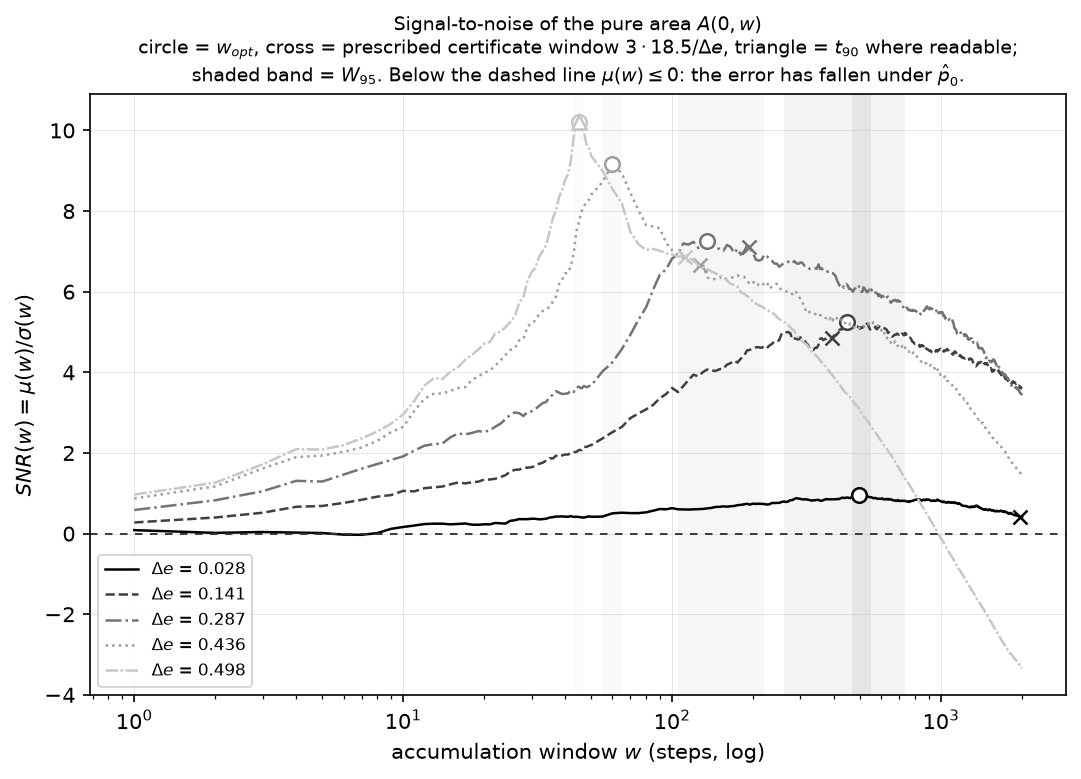
\includegraphics[width=0.85\textwidth]{resultats_R2/resultats/figures/Fig_bis_snr_fenetre.png}
  \caption{$\mathrm{SNR}(w)$ pour cinq amplitudes. La fenêtre de certificat imposée par
  l'énoncé, croix, tombe à droite du maximum à quatre des cinq amplitudes tracées, et à
  gauche à $\Delta e = 0.141$. En haut de grille la courbe passe sous zéro.}
\end{figure}

\clearpage

\section{D.3.bis : la matrice complète, et le paradoxe de Simpson}

\paragraph{Réponse.} Partiellement oui, et la moitié de la démonstration attendue n'est pas
disponible. L'aire sur fenêtre courte est mieux liée que $A(H)$ aux durées de renouvellement
de la forêt : contre $\tau_{\mathrm{ARF}}$, la médiane stratifiée passe de $+0.0526$ pour
$A(H)$, discernable de zéro sur aucune des 18 strates, à $+0.1597$ pour
$A(0,w_{\text{règle}})$, discernable sur 12, et à $+0.2314$ pour $A(0,w_{\mathrm{cert}})$,
discernable sur 13. Contre la date d'alarme du détecteur, en revanche, c'est l'inverse :
$\tau_{\mathrm{det}}(\lambda = 8)$ est discernable sur 5 strates avec $A(H)$ et sur une seule
avec $A(0,w_{\text{règle}})$. Quant à la comparaison qui paraissait la plus directe, celle
des trois aires face à $S_{\max}(H)$ et face à l'aire étalon, elle ne tranche rien : les six
cellules portent le même lien algébrique et sont hachurées.

L'empilement, lui, fabrique de l'association partout : le rapport du coefficient empilé à la
médiane stratifiée vaut $2.9696$ en médiane sur les 55 paires sans lien connu, et cinq paires
changent de signe entre les deux lectures.

\subsection{Périmètre et exclusions}

Douze métriques, 66 paires, en version empilée sur les $2000$ exécutions et stratifiée par
amplitude.\footnote{\texttt{QCD\_bis\_matrice\_correlation.parquet}, une ligne par cellule
avec son intervalle de confiance, son effectif et son taux de censure ;
\texttt{QCD\_bis\_matrice\_resume.parquet} pour le résumé par paire.} Trois grandeurs sont
écartées, avec leur motif : $\tau_{\mathrm{swap}}(10\%)$, identique à $\tau_{\mathrm{ARF}}$ à
$M = 10$ et donc tautologique ; $\tau_{\mathrm{det}}(\lambda = 25)$, censuré à $61.1\%$ ;
$\tau_{\mathrm{det}}(\lambda = 50)$, censuré à $99.95\%$. La seule tautologie connue n'a donc
pas de cellule dans la matrice, et la colonne qui la marquerait y est vide par construction.

\paragraph{Onze cellules portent un lien algébrique connu} et sont hachurées plutôt que lues.
Sept étaient identifiées d'emblée : $(S_{\max}(H), A(H))$ par la forme de Lindley,
$(A(H), \text{étalon})$ et $(S_{\max}(H), \text{étalon})$ par l'identité approchée
$e_t - \hat{p}_0 \approx \Delta e\,(1 - \mathrm{acc})$, $(\int V, \text{étalon})$ par partage
des votes et des sondes, et les trois emboîtements de sommes entre $A(0,w)$ et $A(H)$.

Quatre ont été ajoutées après coup, et c'est la correction la plus lourde de ce document.
$S_{\max}(H) = \max_{k \leq j} [A(k,j) - (j-k)\,\delta_P]$ est un supremum sur une famille
qui contient $A(0,w) - w\,\delta_P$ \emph{pour tout} $w$. Le lien de Lindley ne concerne donc
pas seulement $A(H)$ : il vaut pour chaque $A(0,w)$, et plus étroitement encore pour les
fenêtres courtes, puisque l'argmax de Lindley tombe dans leur voisinage en haut de grille.
Marquer $(S_{\max}, A(H))$ seul revenait à hachurer le terme de comparaison et à inviter à
lire les deux autres. Les cellules $(S_{\max}, A(0,w_{\text{règle}}))$ et
$(S_{\max}, A(0,w_{\mathrm{cert}}))$ sont donc hachurées elles aussi, de même que les deux
cellules de $A(0,w)$ contre l'aire étalon, liées par la même identité approchée que $A(H)$.

Ce marquage retire à D.3.bis la comparaison la plus frappante. Les valeurs restent dans la
table, $+0.7068$ pour $A(0,w_{\mathrm{cert}})$ contre $S_{\max}$, $+0.5954$ pour
$A(0,w_{\text{règle}})$ et $+0.3246$ pour $A(H)$, les 18 strates étant discernables dans les
trois cas ; mais elles ne peuvent pas soutenir un verdict, puisque le lien explique une part
inconnue de l'écart.

\paragraph{Censure.} Une cellule dont l'une des deux marges dépasse $50\%$ de censure dans au
moins une strate du domaine de décision est calculée puis hachurée : onze cellules, toutes
dues aux amplitudes basses. Cette règle ne vaut que pour les cellules neuves ; le contrôle de
non-régression contre la rédaction D garde la définition d'origine, les 18 strates du domaine.
Les deux conventions sont publiées côte à côte : pour la paire
$(\tau_{\mathrm{ARF}}, \tau_{\mathrm{swap}}(75\%))$, la médiane stratifiée vaut $0.097934$ sur
18 strates avec la convention d'origine et $0.090037$ sur 17 avec la règle, soit un rapport
d'amplification de $4.72$ contre
$5.13$.\footnote{\texttt{QCD\_bis\_controle\_conventions.parquet},
\texttt{QCD\_bis\_controle\_censure.parquet}.}

Enfin, $A(0,w_{\text{règle}})$ n'existe qu'aux 18 amplitudes où $t_{1/2}$ est lisible : ses
cellules empilées portent $n = 1800$ et non $2000$, et ses deux strates manquantes sont
grisées.

\subsection{Contrôles}

Le contrôle de non-régression passe exactement : la cellule $(\tau_{\mathrm{ARF}}, A(H))$
redonne $+0.396512$ empilé et $+0.052559$ en médiane stratifiée, rapport $7.54$, valeurs de
\texttt{tab:agregation} de la rédaction D. Le nombre de strates discernables de zéro y est de
$0$ sur $18$, comme dans le rapport.

Pour $(\tau_{\mathrm{ARF}}, S_{\max}(H))$, ce document compte $14$ strates discernables sur
$18$ contre $15$ dans la rédaction D. La différence tient au nombre de rééchantillons,
$1000$ ici contre $2000$ là, et à une graine différente ; elle porte sur une strate dont
l'intervalle frôle zéro et ne change pas le verdict. C'est le chiffre de la rédaction D qui
fait foi, celui-ci étant produit avec moins de rééchantillons.

Le traitement de la censure est contrôlé sur la paire la plus censurée retenue,
$(\tau_{\mathrm{ARF}}, \tau_{\mathrm{swap}}(75\%))$. Sur le domaine de décision, l'écart entre
le coefficient calculé avec imputation à l'horizon et celui calculé sur les cas complets
atteint au plus $0.040259$, à $\Delta e = 0.194$ où la censure vaut $0.13$ ; à l'amplitude la
plus censurée, $\Delta e = 0.141$ et $0.540$ de censure, cet écart n'est que de $0.0087$. Les
deux extrêmes ne tombent donc pas sur la même strate, et le pire écart n'est pas celui de la
pire censure.

Le témoin de Simpson est construit et non emprunté : sur un jeu synthétique où $X$ et $Y$
sont indépendants dans chaque strate mais dont les deux moyennes croissent avec l'indice de
strate, le coefficient empilé vaut $+0.9505$, la médiane stratifiée $+0.0111$ avec un
intervalle $[-0.0188 ; +0.0277]$ qui couvre zéro, et le rapport $85.5467$. Sur le témoin où la
relation est réelle et les moyennes constantes, empilé $+0.5017$ contre stratifié $+0.5032$,
rapport $0.9970$. L'indicateur ne voit Simpson que là où Simpson est. Sa médiane stratifiée
de témoin, $+0.0111$, reste toutefois dix fois plus grande que les dénominateurs les plus
petits rencontrés sur les données : le témoin valide la détection, pas le comportement du
rapport quand le dénominateur s'annule.

Les intervalles de la matrice empilée sont bootstrapés \emph{par grappes de graines} : les 100
graines étant communes aux 20 amplitudes, rééchantillonner les exécutions une à une donnerait
des intervalles trop étroits.

\subsection{Ce que la matrice dit, une fois les cellules liées écartées}

\begin{table}[htbp]
  \centering
  \begin{tabular}{llrrr}
    \toprule
    Comparée à & Métrique d'aire & empilé & médiane stratifiée & strates discernables \\
    \midrule
    $\tau_{\mathrm{ARF}}$ & $A(0,w_{\mathrm{cert}})$  & $+0.3424$ & $+0.2314$ & $13/18$ \\
    $\tau_{\mathrm{ARF}}$ & $A(0,w_{\text{règle}})$   & $+0.4583$ & $+0.1597$ & $12/18$ \\
    $\tau_{\mathrm{ARF}}$ & $A(H)$                    & $+0.3965$ & $+0.0526$ & $0/18$  \\
    \midrule
    $\tau_{\mathrm{swap}}(25\%)$ & $A(0,w_{\text{règle}})$ & $+0.5121$ & $+0.1649$ & $11/18$ \\
    $\tau_{\mathrm{swap}}(25\%)$ & $A(H)$                  & $+0.4567$ & $+0.1240$ & $9/18$  \\
    \midrule
    $\tau_{\mathrm{det}}(\lambda = 8)$ & $A(H)$                  & $+0.3708$ & $+0.0548$ & $5/18$ \\
    $\tau_{\mathrm{det}}(\lambda = 8)$ & $A(0,w_{\text{règle}})$ & $+0.3826$ & $+0.0032$ & $1/18$ \\
    \bottomrule
  \end{tabular}
  \caption{Les seules comparaisons des trois aires qui ne portent pas de lien algébrique
  connu. Les cellules contre $S_{\max}(H)$ et contre l'aire étalon sont hachurées et absentes
  de cette table.}
\end{table}

La validation demandée par le mail est donc acquise du côté de la forêt et refusée du côté du
détecteur. L'aire sur fenêtre courte est bien la meilleure des trois pour ce que
l'adaptation du classifieur laisse fuiter, mesurée par les durées de renouvellement. Elle est
la moins bonne pour prédire quand l'alarme partira, ce qui n'est pas contradictoire :
$A(0,w)$ coupe l'intégration à la fin du transitoire, précisément là où le détecteur, lui,
continue d'accumuler.

Une nuance sur le choix de la fenêtre : celle qui maximise le rapport signal sur bruit de $A$
n'est pas celle qui maximise son pouvoir d'association. La fenêtre de certificat imposée par
l'énoncé, pourtant $1.77$ à $2.49$ fois plus longue que $w_{\mathrm{opt}}$ en haut de grille,
fait aussi bien ou mieux que $w_{\text{règle}}$ contre $\tau_{\mathrm{ARF}}$. Optimiser la
lisibilité d'une grandeur et optimiser son association sont deux problèmes différents, et la
section~\ref{sec:c2bis} répond au premier.

Le fait neuf concerne $\tau_{\mathrm{ARF}}$. Contre $A(H)$, sa médiane stratifiée vaut
$+0.0526$ et aucune des 18 strates n'est discernable de zéro : c'est le verdict du rapport,
inchangé. Contre $A(0,w_{\text{règle}})$, elle vaut $+0.1597$ et 12 strates sur 18 sont
discernables. La date du premier remplacement dit donc quelque chose de l'erreur
\emph{laissée fuiter pendant le transitoire}, alors qu'elle ne dit rien de l'erreur cumulée
sur l'horizon. Cela ne réhabilite pas $\tau_{\mathrm{ARF}}$, l'association restant faible,
mais cela précise contre quoi le verdict négatif de la question D a été rendu.

\subsection{L'ampleur de l'artefact d'agrégation}

Sur les 55 paires sans lien connu, le rapport du coefficient empilé à la médiane stratifiée
vaut $2.9696$ en médiane, et 28 paires gardent au moins la moitié de leurs strates
discernables de zéro. Cinq paires changent de signe entre les deux lectures.

Le maximum, $378.2781$ pour $(\tau_{\mathrm{swap}}(75\%), A(0,w_{\text{règle}}))$, n'est pas
une mesure. Les 18 strates de cette paire vont de $-0.1075$ à $+0.0789$, aucune n'a
d'intervalle excluant zéro, et la série change de signe en cours de grille : la médiane
$0.001113$ est le point où deux valeurs opposées se croisent, pas une estimation. Le rapport
y est donc un artefact de dénominateur, et il est instable en conséquence : sous la
convention réservée aux cellules neuves, qui écarte la strate trop censurée, la médiane vaut
$0.002023$ et le rapport $208.05$. Ces valeurs se lisent comme une direction, pas comme une
grandeur. La médiane des 55 paires, elle, ne bouge pas de façon sensible entre les deux
conventions.

Le deuxième plus fort, $118.3557$ pour
$(\tau_{\mathrm{det}}(\lambda = 8), A(0,w_{\text{règle}}))$, a le même défaut, avec une seule
strate discernable sur 18. Aucun coefficient empilé n'est cité comme résultat dans ce
document ni dans le rapport : la matrice empilée est montrée pour être réfutée par la
stratifiée.

\begin{figure}[htbp]
  \centering
  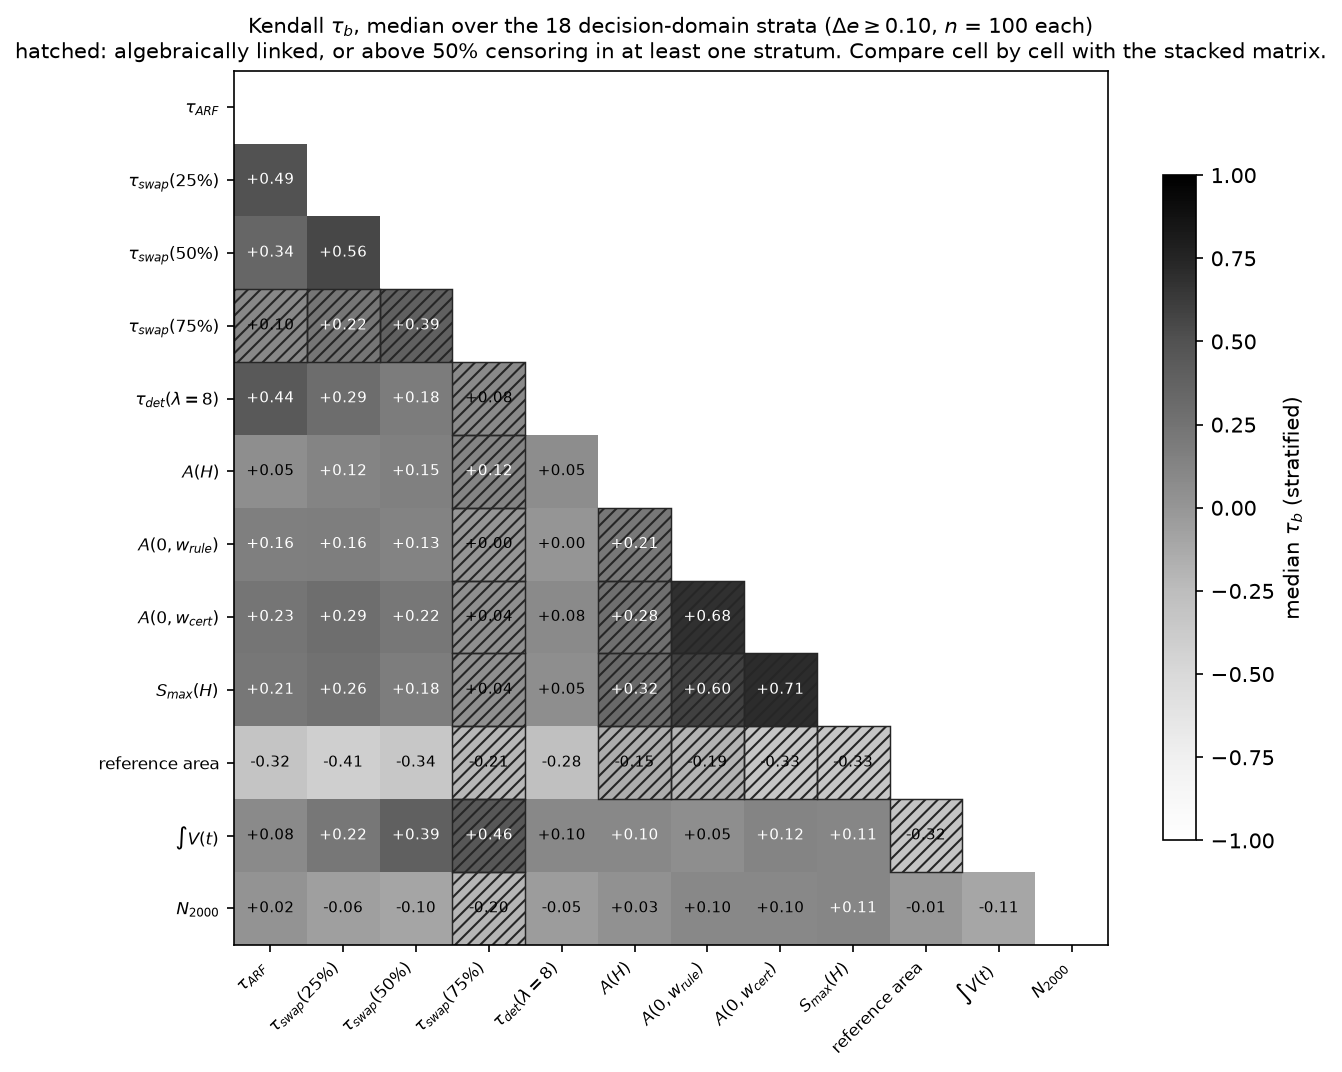
\includegraphics[width=0.92\textwidth]{resultats_R2/resultats/figures/Fig_bis_matrice_stratifiee_mediane.png}
  \caption{Médiane des $\tau_b$ sur les 18 strates du domaine de décision. Les cellules
  hachurées portent un lien algébrique, ou plus de $50\%$ de censure dans au moins une strate.}
\end{figure}

\begin{figure}[htbp]
  \centering
  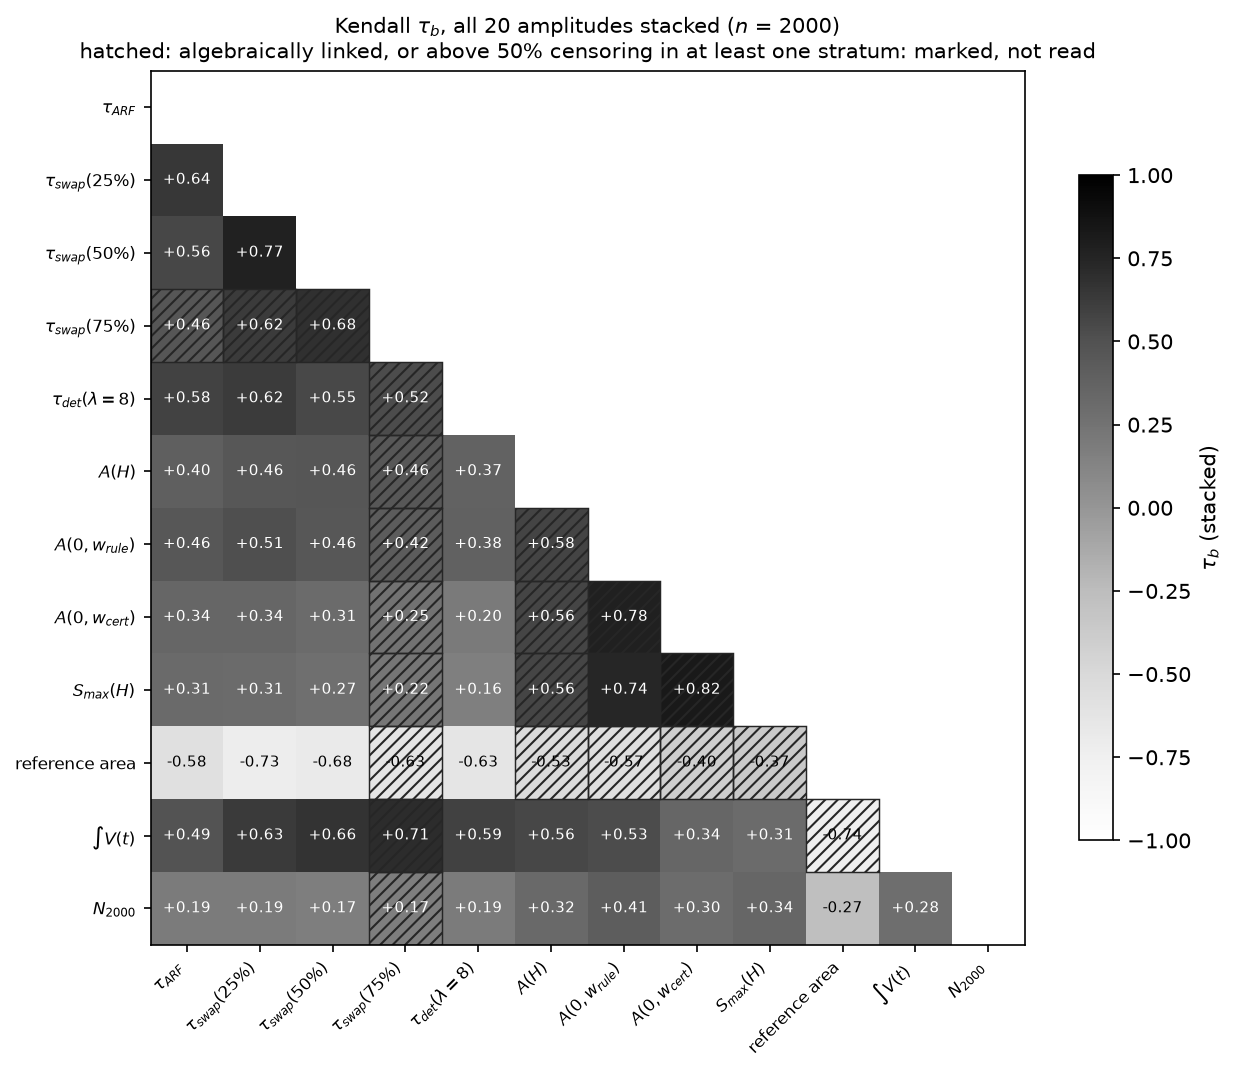
\includegraphics[width=0.92\textwidth]{resultats_R2/resultats/figures/Fig_bis_matrice_empilee.png}
  \caption{La même matrice, toutes amplitudes empilées. À comparer cellule à cellule avec la
  précédente.}
\end{figure}

\begin{figure}[htbp]
  \centering
  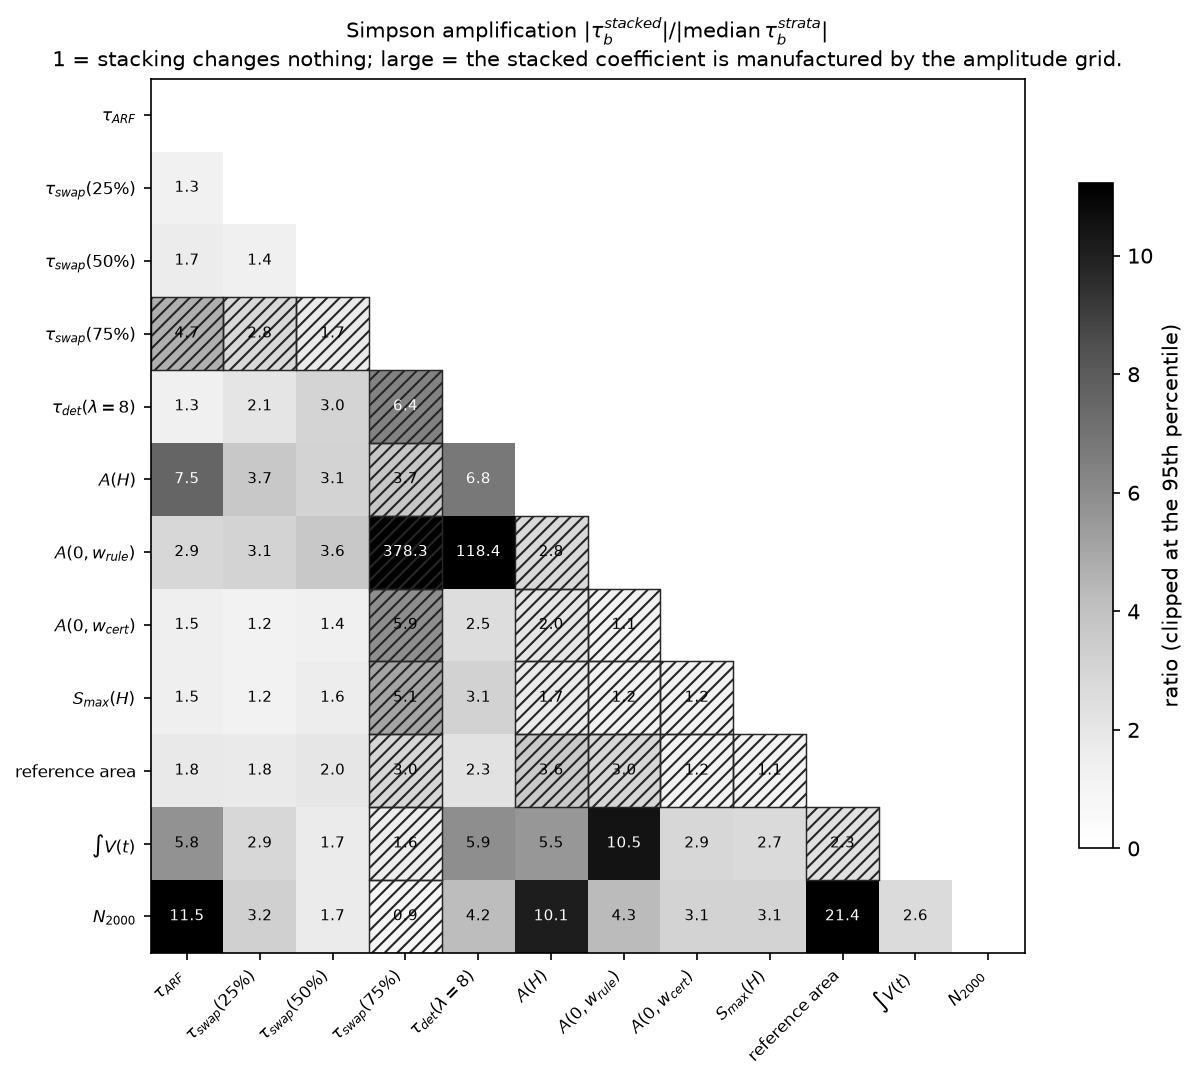
\includegraphics[width=0.92\textwidth]{resultats_R2/resultats/figures/Fig_bis_matrice_ratio_simpson.png}
  \caption{Rapport des deux lectures. Une valeur de $1$ signifie que l'empilement ne change
  rien ; les valeurs élevées marquent les paires dont le coefficient global est fabriqué par
  la grille d'amplitudes, y compris celles dont la médiane stratifiée n'est pas discernable de
  zéro, où le rapport n'a pas de contenu.}
\end{figure}

\begin{figure}[htbp]
  \centering
  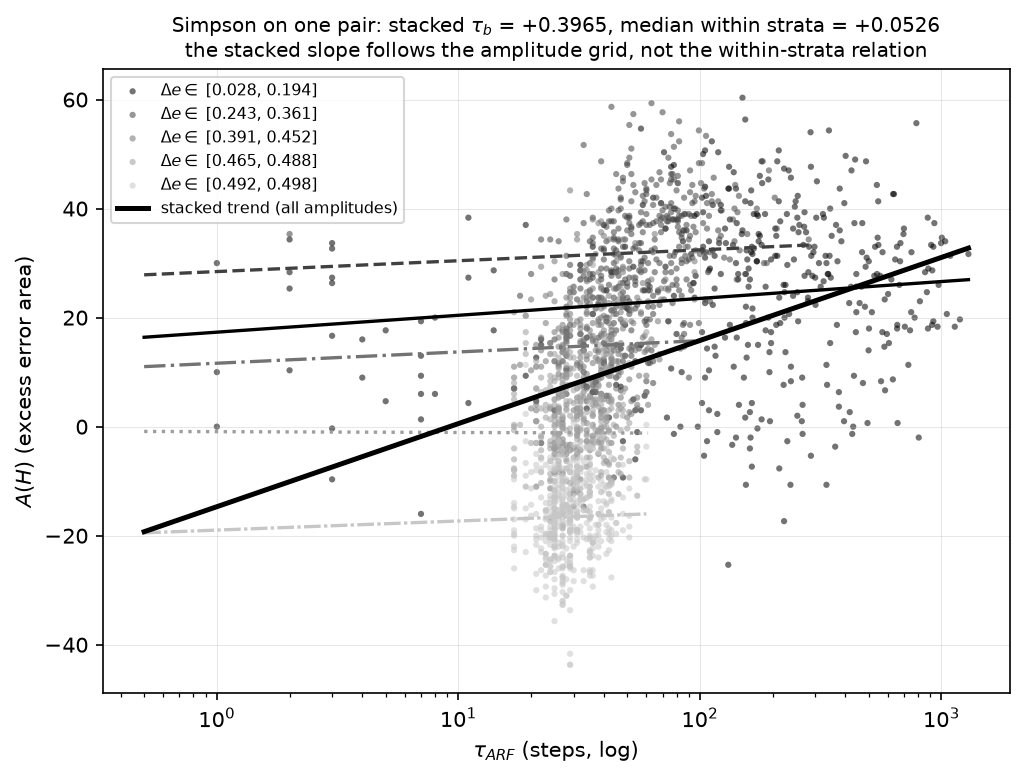
\includegraphics[width=0.82\textwidth]{resultats_R2/resultats/figures/Fig_bis_simpson_paire.png}
  \caption{Le paradoxe sur une paire. La pente empilée suit l'alignement des nuages par
  amplitude, pas la relation à l'intérieur de chacun. Chaque droite est ajustée et tracée sur
  l'étendue de son propre groupe.}
\end{figure}

\clearpage

\section{D.1.bis : ce qui se passe entre les arbres}
\label{sec:d1bis}

\paragraph{Réponse.} La forêt ne se répare pas seulement en remplaçant des arbres. Le
désaccord entre arbres retombe à mi-hauteur alors que la fraction d'arbres distincts
renouvelés ne vaut que $0.6320$ à $0.6650$ sur les huit amplitudes les plus fortes : les
survivants apprennent. Et le pilote instrumenté renverse l'hypothèse de départ. Après une
forte rupture, les arbres neufs ne sont pas les mauvais élèves de la forêt, ils en sont les
meilleurs : leur taux d'erreur vaut $0.0050$ contre $0.2270$ pour les survivants à
$\Delta e = 0.498$. L'effet Hydre n'est pas une dégradation causée par des arbres jeunes,
c'est un retard causé par des arbres âgés que le drift a rendus faux.

\subsection{Le constat, avant toute mesure}

Aucune table de la campagne ne porte l'erreur d'un arbre à un pas donné.
\texttt{exp\_QCD\_campagne.py} n'enregistre que l'erreur de la forêt et les événements de
remplacement ; \texttt{exp\_QCD\_etalon.py} interroge bien chaque arbre, mais somme
immédiatement sur les 10 arbres et les 200 sondes. La variance en coupe transversale demandée
par le mail n'était donc calculable depuis aucun Parquet.

Un second argument limite ce qu'une variance instantanée peut apprendre. Sur des erreurs
binaires $e_m(t) \in \{0,1\}$, la variance entre les $M$ arbres à un instant donné vaut
$\bar{p}_t(1-\bar{p}_t)$ au facteur $M/(M-1)$ près, où $\bar{p}_t$ est la fraction d'arbres
en erreur ; le désaccord avec la majorité vaut $\min(\bar{p}_t, 1-\bar{p}_t)$. Les deux sont
la même grandeur à une transformation monotone près. Ce qu'aucune des deux ne voit, et qui
fait l'effet Hydre, est l'hétérogénéité \emph{persistante} des taux d'erreur par arbre. Elle
exige des traces par arbre.

\subsection{Le proxy disponible, et ses limites}

$V(t)$, le désaccord instantané mesuré tous les 25 pas sur les sondes de l'étalon, est
disponible sans resimuler.\footnote{\texttt{QCD\_bis\_dispersion\_arbres.parquet}.} Il partage
ses votes, ses sondes et sa fenêtre avec l'aire étalon : ce n'est pas une mesure externe, et
ce point est repris en section~\ref{sec:nonfait}. Le pas de sonde de 25 ne résout pas la
montée en haut de grille, où $\tau_{\mathrm{ARF}}$ médian vaut $28$ pas.

Dans la bande où le drift agit, $V(t)$ monte de $0.0516$ à $t = 0$ jusqu'à un pic de $0.2803$
à $t = 50$ à $\Delta e = 0.498$, puis retombe. Le fait à retenir est la date de cette
retombée rapportée au renouvellement : $V$ revient à mi-hauteur alors que la fraction
d'arbres distincts remplacés vaut $0.6410$. La forêt s'est déjà réaccordée pour moitié avec
un tiers de ses arbres d'origine encore en place.

\subsection{Le pilote instrumenté}

Le proxy ne répondant pas à la question posée, un pilote a été lancé : 5 amplitudes,
20 graines, $M = 10$, horizon $2000$, soit 100 exécutions en $1.1$
minute.\footnote{\texttt{QCD\_bis\_pilote\_arbres\_pilote.log}, log de campagne, avec la
grille, les graines, la durée et le résultat du contrôle.} C'est une campagne, décidée avec
son coût, pas une vérification. Le contrôle exigé avant lecture est passé : sur les 100
exécutions, la trajectoire d'erreur de la forêt reproduit \texttt{QCD\_traces\_error\_full}
sans un seul pas différent, et les événements de remplacement coïncident un à un. Le sondage
par arbre n'a donc consommé aucun
aléa.\footnote{\texttt{QCD\_bis\_traces\_arbres\_pilote.parquet},
\texttt{QCD\_bis\_variance\_arbres.parquet},
\texttt{QCD\_bis\_variance\_arbres\_agregee.parquet}.}

Les taux d'erreur par arbre sont lus sur des blocs alignés sur le $\tau_{\mathrm{ARF}}$
\emph{de chaque exécution}, $[k\,\tau_{\mathrm{ARF}}, (k+1)\,\tau_{\mathrm{ARF}})$, et non sur
une fenêtre fixe : une fenêtre de 50 pas décalerait de 25, contre un transitoire de 28 à 38
pas en haut de grille. Les blocs $0$ et $1$ ne comptent aucun arbre remplacé : le bloc $0$
s'arrête avant le premier remplacement par définition de $\tau_{\mathrm{ARF}}$, et le bloc $1$
commence à cet instant, si bien que l'état lu à son début est encore vierge. La colonne des
arbres neufs y est donc vide.

\begin{table}[htbp]
  \centering
  \begin{tabular}{lrrrrr}
    \toprule
    $\Delta e$ & bloc & variance entre arbres & excès sur l'échantillonnage
    & taux des neufs & taux des survivants \\
    \midrule
    $0.028$ & $0$ & $0.0026$ & $1.8821$ & indéfini & $0.0743$ \\
    $0.028$ & $2$ & $0.0035$ & $3.3855$ & $0.1426$ & $0.0694$ \\
    $0.416$ & $0$ & $0.0052$ & $0.5027$ & indéfini & $0.4140$ \\
    $0.416$ & $2$ & $0.0070$ & $1.6958$ & $0.1069$ & $0.2139$ \\
    $0.498$ & $0$ & $0.0064$ & $0.4615$ & indéfini & $0.4716$ \\
    $0.498$ & $2$ & $0.0185$ & $6.6924$ & $0.0050$ & $0.2270$ \\
    \bottomrule
  \end{tabular}
  \caption{Variance transversale des taux d'erreur par arbre, blocs alignés sur
  $\tau_{\mathrm{ARF}}$. L'excès est le rapport de la variance observée à celle qu'un
  échantillonnage pur donnerait si tous les arbres avaient le même taux. Les blocs $4$ et $5$
  de $\Delta e = 0.028$ reposent sur $18$ et $17$ exécutions, les autres sur $20$ : à cette
  amplitude $\tau_{\mathrm{ARF}}$ est assez long pour que six blocs dépassent l'horizon.}
\end{table}

Trois lectures. D'abord, dans le bloc 0, avant tout remplacement, la variance observée est
\emph{inférieure} à celle d'un échantillonnage indépendant en haut de grille, $0.4615$ à
$\Delta e = 0.498$ : les arbres voient les mêmes points et se trompent ensemble. Ce rapport
n'est pas un test, c'est un repère.

Ensuite, l'excès dépasse $1$ à tous les blocs à partir du bloc $1$, et monte à $6.6924$ au
bloc $2$ à $\Delta e = 0.498$ : l'hétérogénéité entre arbres devient réelle et persistante,
pas un artefact d'échantillonnage. C'est ce que la variance instantanée ne pouvait pas voir.
Le remplacement n'en a pas pour autant l'exclusivité : en bas de grille, à
$\Delta e = 0.028$, l'excès vaut déjà $1.8821$ au bloc $0$, avant qu'un seul arbre ait été
remplacé. Les quatre blocs $0$ d'excès inférieur à $1$ sont tous à $\Delta e \geq 0.243$.

Enfin, le signe de l'écart entre arbres neufs et survivants s'inverse le long de la grille. À
$\Delta e = 0.498$ les neufs valent $0.0050$ contre $0.2270$ aux survivants, un écart de
$-0.2220$. À $\Delta e = 0.028$ l'écart vaut $+0.0732$, les neufs étant alors les plus
mauvais. La lecture est cohérente avec un acquis du journal, selon lequel la tâche devient
plus facile après une forte rupture : un arbre neuf apprend directement la nouvelle règle, un
survivant traîne l'ancienne. En bas de grille, où le remplacement est déclenché par le bruit,
il détruit de l'information au lieu d'en apporter.

\begin{figure}[htbp]
  \centering
  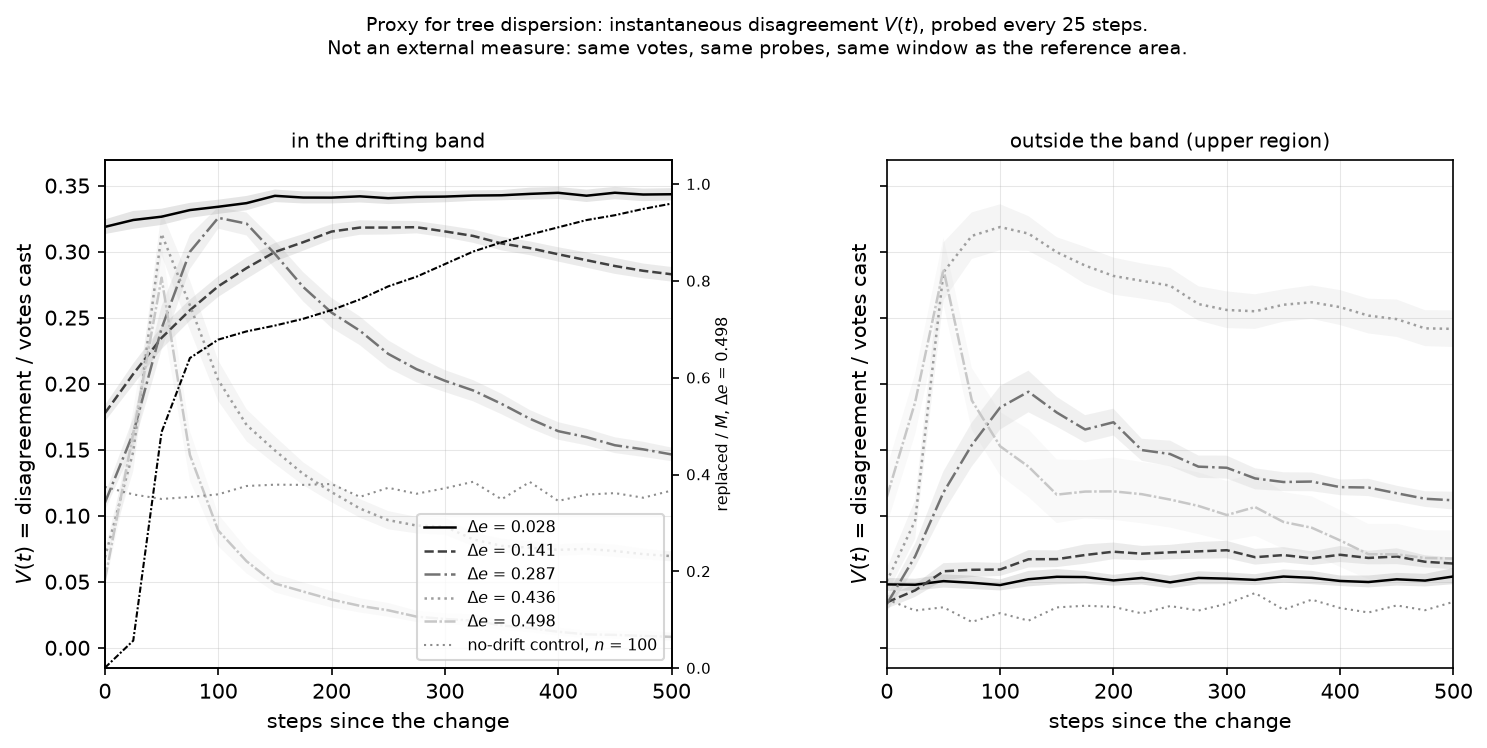
\includegraphics[width=\textwidth]{resultats_R2/resultats/figures/Fig_bis_dispersion_arbres.png}
  \caption{Proxy $V(t)$, désaccord instantané, dans la bande et hors bande, avec la fraction
  d'arbres distincts remplacés. Témoin sans drift sur 100 exécutions.}
\end{figure}

\begin{figure}[htbp]
  \centering
  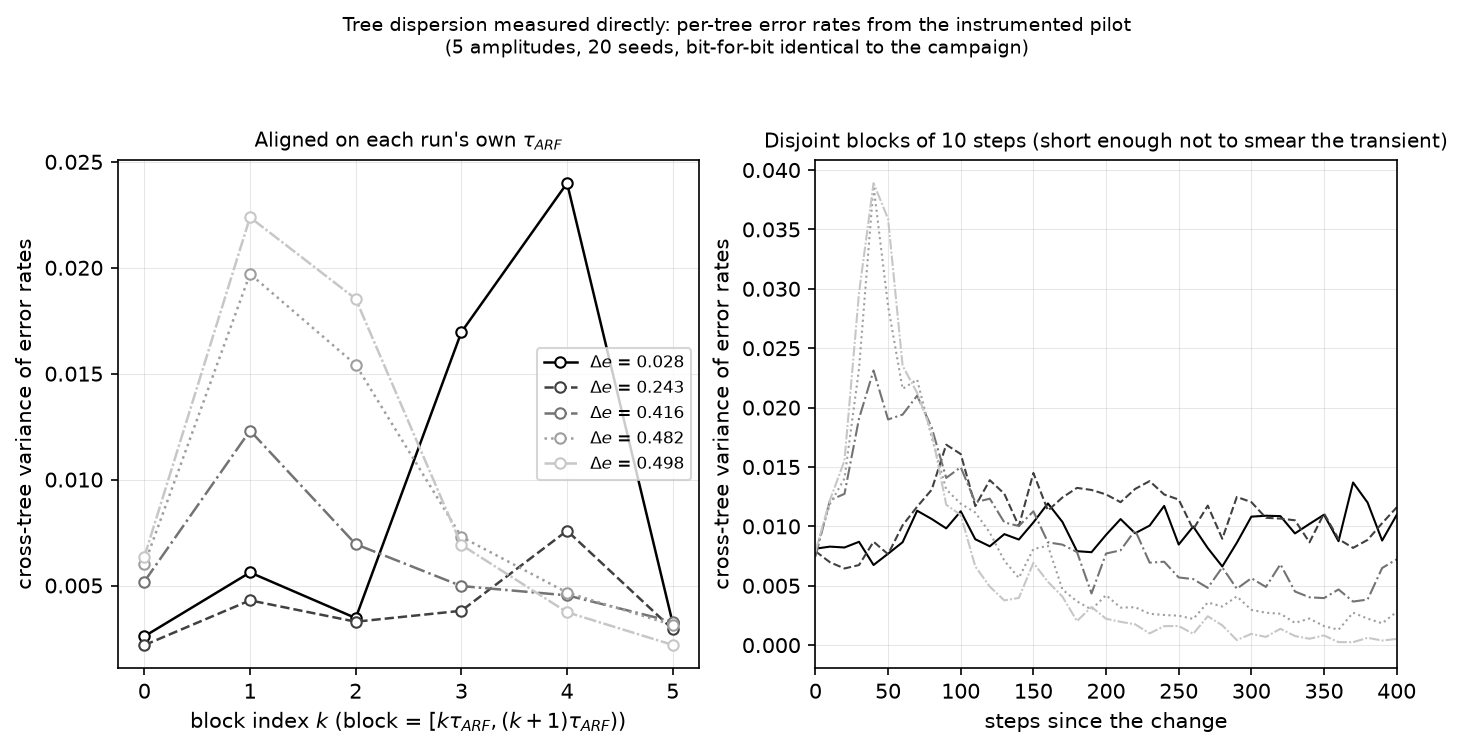
\includegraphics[width=\textwidth]{resultats_R2/resultats/figures/Fig_bis_variance_arbres.png}
  \caption{Variance transversale mesurée directement sur le pilote instrumenté. À gauche par
  blocs alignés sur $\tau_{\mathrm{ARF}}$, à droite par blocs disjoints de 10 pas.}
\end{figure}

\clearpage

\section{C.1.bis : le Z-score de la baisse d'erreur}

\paragraph{Réponse.} Négative, et l'encadrant a raison de la placer en dernier. L'instant où
le Z-score franchit un seuil mesure le nombre de graines moyennées, pas la dynamique de la
forêt. À $\Delta e = 0.141$ et au seuil $3$, il vaut $751$ pas avec 25 graines, $487$ avec 50
et $353$ avec 100.\footnote{\texttt{QCD\_bis\_t\_zscore.parquet}.} Le dénominateur décroît en
$1/\sqrt{n}$ : ajouter des graines fait franchir le seuil plus tôt, à dynamique strictement
inchangée. Le même effet joue sur le seuil : à la même amplitude et avec 100 graines, $230$,
$353$ et $529$ pas pour les seuils $2$, $3$ et $4$.

Trois amplitudes ne font pas une démonstration, aussi la dépendance est-elle mesurée sur
toute la grille. En rapportant $t_Z(n)$ à $t_Z(100)$ pour chaque amplitude où l'instant
existe aux trois tailles, la médiane vaut $1.3333$, $1.3516$ et $1.4091$ à $n = 25$ pour les
seuils $2$, $3$ et $4$.\footnote{\texttt{QCD\_bis\_zscore\_rapports.parquet}.} Le sens est le
même sur $18$ des $19$ amplitudes au seuil $2$, et sur la totalité des $18$ et des $17$
amplitudes aux seuils $3$ et $4$.

La décroissance n'est pas universelle pour autant. Sur les $54$ triplets, deux ne sont pas
monotones : à $\Delta e = 0.085449$ et au seuil $2$, $t_Z$ passe de $534$ à $618$ entre 25 et
50 graines avant de redescendre à $609$ ; à $\Delta e = 0.242568$ et au même seuil, de $112$ à
$123$ puis $92$. Les deux sont au seuil le plus bas, celui où le franchissement est le plus
bruité.

À $\Delta e = 0.028$, aucune des neuf combinaisons de seuil et de taille d'échantillon ne
donne d'instant défini : la baisse d'erreur y vaut $0.002$, sous le bruit.

La version invariante en $n$ du même objet existe déjà : c'est le premier instant où la
baisse dépasse une fraction déclarée de $e_{\mathrm{start}} - e_\infty$, c'est-à-dire
$t_{25}$, $t_{1/2}$ et $t_{90}$ de la section~1. Ces trois-là ne dépendent pas du nombre de
graines, seulement leur incertitude en dépend, ce qui est le comportement attendu d'un
estimateur.

\begin{figure}[htbp]
  \centering
  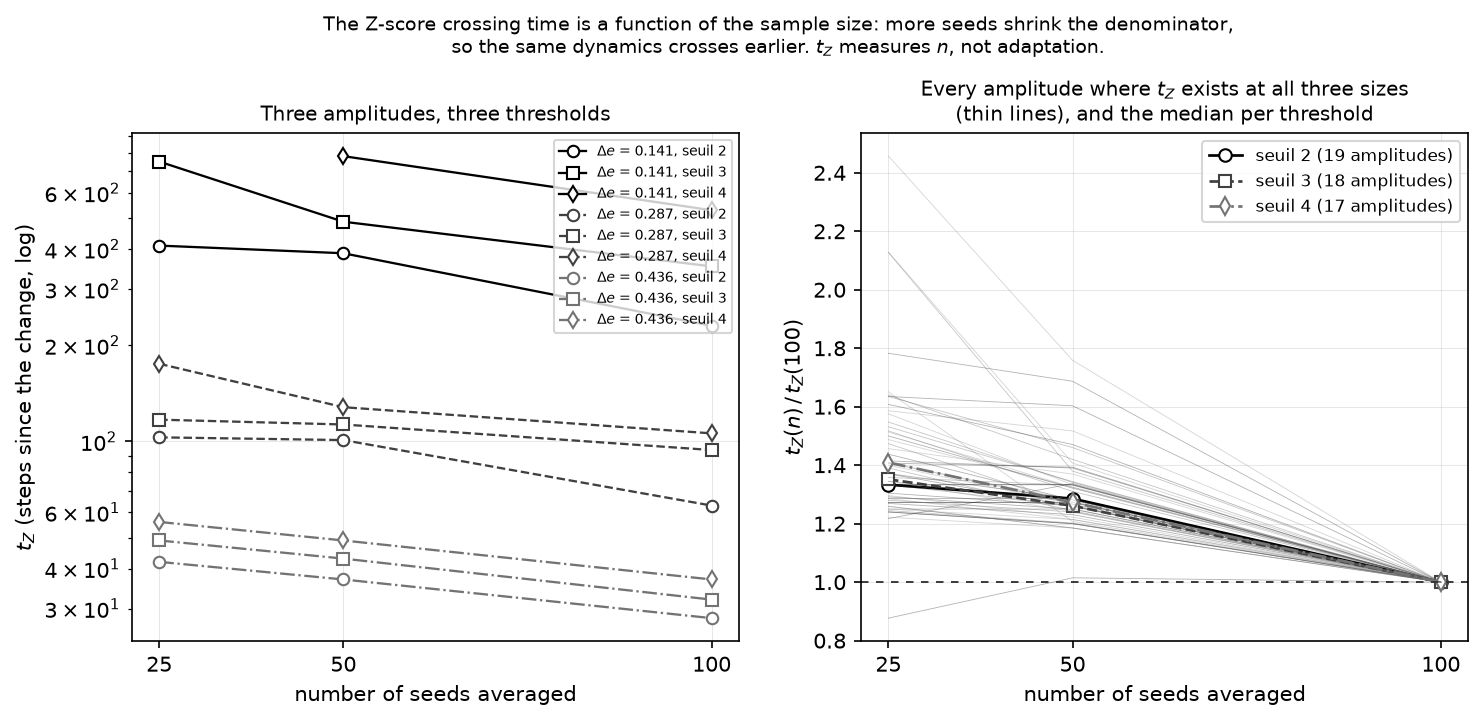
\includegraphics[width=\textwidth]{resultats_R2/resultats/figures/Fig_bis_zscore.png}
  \caption{$t_Z$ en fonction du nombre de graines moyennées. À gauche trois amplitudes et
  trois seuils ; à droite toutes les amplitudes, rapportées à leur valeur à $n = 100$. Une
  grandeur qui décroît quand on ajoute des observations ne mesure pas le phénomène.}
\end{figure}

\section{Ce qui n'a pas été fait}
\label{sec:nonfait}

\begin{itemize}
  \item \textbf{Les énoncés complets des cinq questions n'ont pas été lus.} Le fichier reçu
  est le corps du mail ; les réponses suivent ce texte, et peuvent manquer une exigence
  formulée en pièce jointe.

  \item \textbf{$S_{\max}(H)$ n'est pas un terme de comparaison indépendant de $A(0,w)$.}
  C'est un supremum sur une famille qui contient $A(0,w) - w\,\delta_P$ pour tout $w$. La
  comparaison des trois aires face à lui est donc en partie algébrique, dans les deux sens,
  et la section~3 ne s'en sert plus pour trancher. La même réserve vaut pour l'aire étalon,
  liée aux trois par l'identité approchée $e_t - \hat{p}_0 \approx \Delta e\,(1 - \mathrm{acc})$.

  \item \textbf{Le verdict de forme de C.3.bis et son critère de sélection vont dans le même
  sens.} Le rapport $t_{90}/t_{1/2}$ décroît avec l'amplitude, et le critère de lisibilité ne
  se lève qu'en haut de grille : les huit amplitudes retenues sont celles où le rapport est le
  plus bas. Le compte de huit bascule à sept ou neuf pour deux décimales de bruit.

  \item \textbf{$e_\infty$ est déclaré non fiable à $\Delta e = 0.390998$ et
  $\Delta e = 0.465040$.} La seconde est l'une des huit amplitudes du test de forme, et c'est
  d'elle que vient la borne haute $1.9714$ citée en section~1. Tous les $t_q$ étant définis
  relativement à $e_\infty$, cette réserve se propage à eux.

  \item \textbf{Le rapport d'amplification de Simpson n'est pas borné} quand la médiane
  stratifiée n'est pas discernable de zéro. Son maximum se lit comme une indication de
  direction, pas comme une mesure, et le témoin synthétique ne couvre pas cet ordre de
  grandeur de dénominateur.

  \item \textbf{La variance par arbre n'est mesurée que sur un pilote}, 5 amplitudes et 20
  graines, contre 20 et 100 pour la campagne. Les écarts entre arbres neufs et survivants ne
  portent donc pas d'intervalle de confiance comparable à celui des autres résultats du
  rapport, et les amplitudes intermédiaires ne sont pas couvertes.

  \item \textbf{La multiplicité n'est pas corrigée.} La matrice stratifiée compte 66 paires
  sur 18 strates, soit $1188$ coefficients. Aucune correction de Bonferroni ni de taux de
  fausses découvertes n'est appliquée : seules les cellules dont l'intervalle est loin de zéro
  se citent, ce qui est une règle de lecture, pas un contrôle.

  \item \textbf{$N_{2000}$ figure dans la matrice alors que le journal le déclare non
  tranché.} Le nombre de remplacements sur l'horizon complet y est noté anti-informatif, le
  drift en produisant moins que son absence, sans que la cause soit établie. Ses onze cellules
  sont calculées et publiées, mais aucune n'est lue comme un résultat.

  \item \textbf{$w_{\text{règle}}$ dérive d'un cas fermé que les données réfutent.} La
  relation $w_{\mathrm{opt}} = 1.2564\,\theta$ suppose un bruit d'écart-type constant ; le
  contrôle sur cas connu montre que la vérité vaut $2.85\,\theta$ pour un bruit binomial. Le
  seul mérite de cette fenêtre est de ne pas être choisie sur les graines qui servent ensuite
  à la corrélation.

  \item \textbf{Le témoin à bruit corrélé ne reproduit pas l'amplitude du régime des
  données}, seulement son sens. La couverture de $W_{95}$ validée sur lui ne transporte donc
  pas telle quelle.

  \item \textbf{Le témoin sans drift de C.3.bis tourne sur $2000$ graines}, la mesure sur
  $100$ par strate. Il ne teste pas le régime de bruit dans lequel $t_q$ est calculé.

  \item \textbf{$V(t)$ n'est pas une mesure externe.} Il partage votes, sondes et fenêtre avec
  l'aire étalon. Une dispersion mesurée sur un dispositif indépendant reste à faire.

  \item \textbf{$t_{90}$ n'est lisible qu'aux huit amplitudes les plus fortes}, et le verdict
  de forme ne vaut que là. Aux douze autres, la table le porte, grisé.

  \item \textbf{Le biais de la règle de franchissement n'est pas corrigé, seulement
  mesuré} : environ la moitié de la fenêtre de persistance sur le cas connu. Tous les $t_q$
  publiés le portent.

  \item \textbf{Les graines sont communes aux vingt amplitudes.} Les comparaisons entre
  amplitudes sont donc appariées, ce qui est déclaré et traité par un bootstrap par grappes de
  graines sur la matrice empilée, mais reste une dépendance que les strates prises isolément
  ignorent.
\end{itemize}

\end{document}
